\documentclass[a4paper,aps,prl,12pt,tightenlines,superscriptaddress]{revtex4}
\usepackage[top=1in,
bottom=1in,
left=1in,
right=1in]{geometry}

\usepackage{natbib}
\usepackage{multirow}
\usepackage{graphicx}
\usepackage{tipa}
\usepackage{marvosym}
\usepackage{color}
\usepackage{placeins}
\usepackage{tabularx, ragged2e,booktabs, caption}
\usepackage[utf8]{inputenc}
\usepackage{gb4e}
\usepackage[T1]{fontenc}
\usepackage{ tipa }
\usepackage{hyperref}
\bibpunct[: ]{(}{)}{,}{a}{}{,}

\newcommand{\noteme}[1]{\noindent \textbf{[[JCW:  #1 ]]}}

\title{}
%\author{}
%\date{}

\begin{document}

\begin{center} \textbf{Allophonic Emergence: three ways allophonic rules come to be} \\
 New Ways of Analyzing Variation workshop submission
 \end{center}

%\maketitle


We are now reaching the point in the fields of language change, sociolinguistics, and language acquisition where we can go well beyond Neogrammarian descriptions of sound change to ask nuanced questions about how phonological systems emerge, and model how grammatical, acquisitional, and mechanical factors create different possible outcomes of change. Aided by increasing higher quality quantitive data on sound change in progress, we have the opportunity to build on important advances to the theory of language change such as \citet{kiparsky1995b} and \citet{labov1994}, and develop hypotheses about the origins of phonological change and the mathematical patterns different types of changes create. This is to say that we can now treat the ``actuation problem'' as more than just a problem \citep{wlh1968}: it is a research program. In this paper, we consider the actuation of allophonic splits, and argue that there are at least three distinct scenarios which can result in allophony during the acquisition process.

The three possible diachronic paths to allophony, which we believe are all currently attested, are the following:

\textbf{Mechanical Means:} This is the traditionally assumed scenario, first stated in terms of modern articulatory phonetics in \citet{ohala1983, ohala1989}. We follow \citet[][and previous work]{bermudezotero2014}'s understanding of this type of change: a mechanical, sub-grammatical articulatory or perceptual effect created by an adjacent phonetic environment skews the distribution of phonetic outputs perceived by the learner. If the skewing is strong enough, part of the distribution is eventually reanalyzed as a different phonological category, an allophone which surfaces by rule (or constraint) in the phonological environment which originally created the phonetic skewing. Thus an originally phonetic effect is phonologized. We believe the emergence of preaspiration as a phonological rule, in varieties like Icelandic and Northwest England English, is an example of this kind of change \citep{Hejna2014}.

\textbf{Spontaneous phonologization:} Speakers spontaneously create an allophone without any phonetic motivation: speakers split one phonological category into two through a pure reanalysis, creating an allophone with no initial phonetic difference from the other allophone. Subsequently, over generational time, the two purely phonological allophones diverge phonetically. Fruehwald (2013) provides an example of spontaneous phonologization in the \textsc{price} split in Philadelphia, providing evidence that the reanalysis of pre-voiceless \textsc{price} and pre-elsewhere \textsc{pride} preceded \textsc{price}-raising in the community.

%\floatbarrier
\textbf{Phonological Specialization:} %A purely phonetic change begins, creating variation in phonetic space, and then different sections of this variation begin to specialize for different phonological contexts over time. The phonological change occurs as a reanalysis of the ``old'' and ``new'' variants of a phonetic change in progress, after that change is well underway (for independent reasons). 
A purely phonetic change begins, creating variation in phonetic space. This variation become reanalyzed as distinct allophonic variants for a given generation of speakers. We see an example of allophonic specialization in \textsc{goose}-fronting in New Zealand English, with \textsc{goose} beginning to front as a single variant which then splits into preceding yod \textsc{new} and non-yod \textsc{goose} words (see Figure 1). We argue that this is distinct from the traditionally mechanical means of allophonic split in production as well as in the predictions about possible conditioning environments.

Finally, we note that even distinguishing these different pathways of change would not be possible without the precise level of observation and replicability large sociolinguistic corpora provide us. We hope that these increasingly precise hypotheses will spark new phonological research using such corpora which will ultimately falsify or improve them.

\begin{figure}
\begin{center}
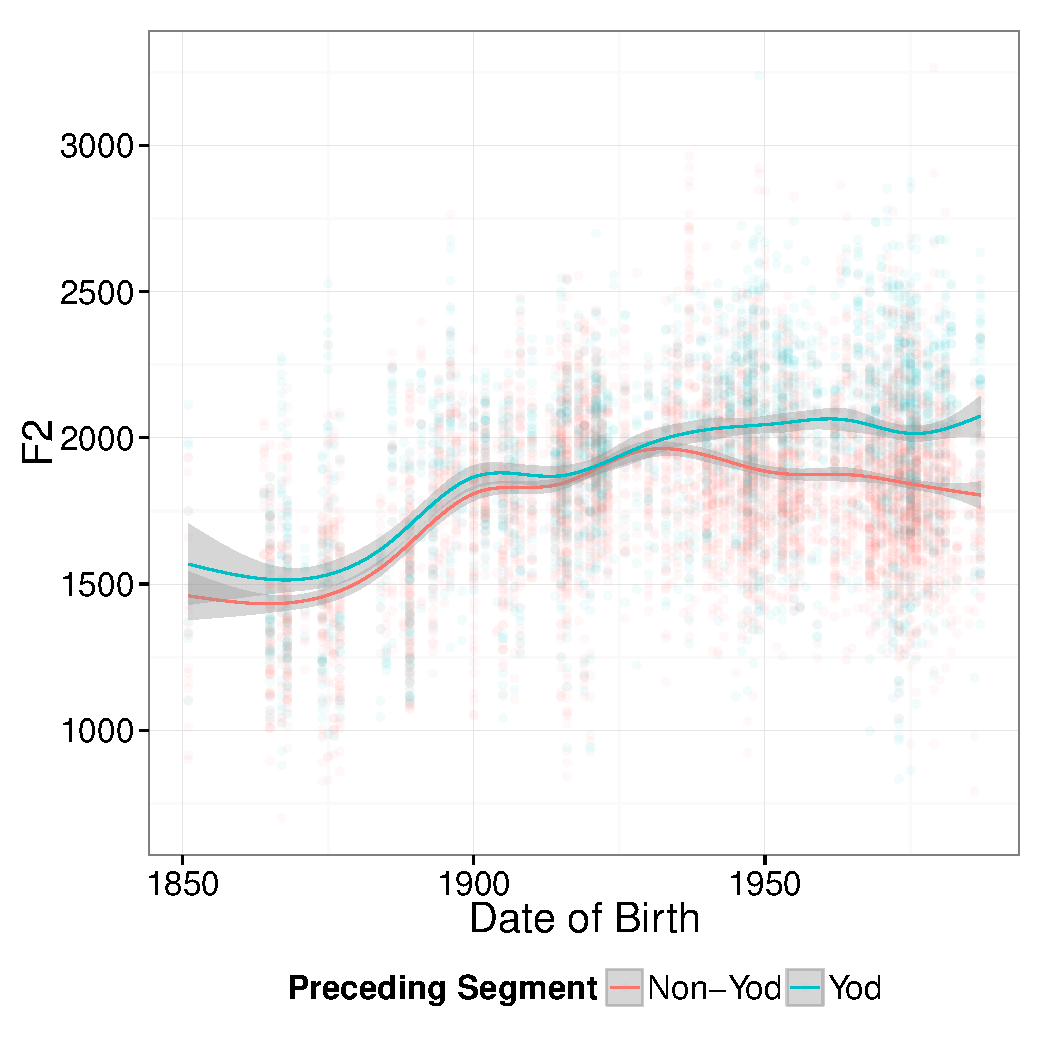
\includegraphics[width=.7\textwidth]{ByTokenOldPreceding.pdf}
\end{center}
\caption{Phonological specialization type allophonic split in New Zealand English GOOSE}
\label{newzeaFig}
\end{figure}

%\floatbarrier

Each of these three pathways to allophonic split make distinct predictions about the production and perception of the variants involved. We present evidence suggesting that all of these scenarios have occurred in the histories of languages, and suggest a research program to distinguish these three scenarios in production data. 

%Rather, we intend to present discussion as a challenge to the fields of historical phonology and sociolinguistics to either confirm or falsify these hypotheses, or to show that some of these scenarios can in fact be reduced to one of the others. 

\bibliographystyle{linquiry2} 
\bibliography{../tyneside/articles/joelrefs}

\end{document}